\documentclass{beamer}

\usepackage[utf8]{inputenc}
\usecolortheme{beaver}
\usepackage{caption}
\usepackage{subcaption}
\usepackage{mathtools}
\usepackage{todonotes}
\usepackage{amsmath}
\usepackage{bm}
\usepackage{listings}
\usepackage{ragged2e}
\usepackage{titlecaps}
\usepackage{fancyvrb}

\def\ci{\perp\!\!\!\!\!\perp}

\newtheorem{proposition}{Proposition}
\Addlcwords{for a is but and with of in as the etc on to if}

\setbeamertemplate{section in toc}{\inserttocsectionnumber.~\inserttocsection}
\usetheme{Boadilla}
\makeatletter
\setbeamertemplate{footline}{%
    \leavevmode%
    \hbox{%
        \begin{beamercolorbox}[wd=.3\paperwidth,ht=2.25ex,dp=1ex,center]{author in head/foot}%
            \usebeamerfont{author in head/foot}\insertshortauthor\expandafter\beamer@ifempty\expandafter{\beamer@shortinstitute}{}{~~(\insertshortinstitute)}
        \end{beamercolorbox}%
        \begin{beamercolorbox}[wd=.55\paperwidth,ht=2.25ex,dp=1ex,center]{title in head/foot}%
            \usebeamerfont{title in head/foot}\insertshorttitle
        \end{beamercolorbox}%
        \begin{beamercolorbox}[wd=.15\paperwidth,ht=2.25ex,dp=1ex,right]{date in head/foot}%
            \usebeamerfont{date in head/foot}\insertshortdate{}\hspace*{2em} \insertframenumber{} / \inserttotalframenumber\hspace*{2ex} 
        \end{beamercolorbox}}%
        \vskip0pt%
    }
\makeatother

\begin{document}

\title[]{Self-Compatibility: Evaluating Causal Discovery without Ground Truth}
\date{}

\begin{frame}
	\begin{figure}
		\includegraphics[scale=0.15]{imgs/title.png}
	\end{figure}
\end{frame}

\begin{frame}{Directed Acyclic Graphs (DAGs)}
	\begin{columns}
		\begin{column}{0.55\textwidth}
		\begin{itemize}
			\item Nodes represent random variables.
			\item Edges represent causal relationships.
			\item E.g., \textbf{Education} has a direct effect on \textbf{Income}. 
			\item E.g., \textbf{Age} has indirect effect on \textbf{Income} through \textbf{Education} and \textbf{Hours Per Week}.
			\item Used for causal effect estimation.
		\end{itemize}
		\end{column}

		\begin{column}{0.45 \textwidth}
		\begin{figure}
			\centering
			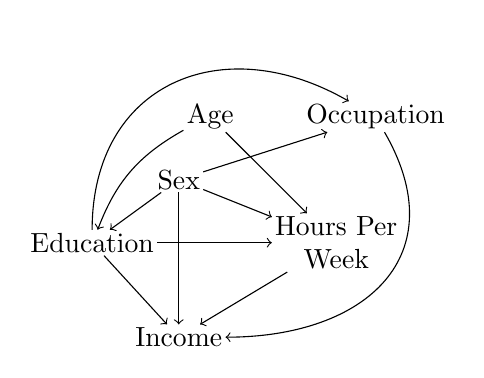
\begin{tikzpicture}[scale=1]
			\tikzstyle{every node}=[align=center, inner sep=1pt]
				\node (sex) at (-0.7, -0.8) {Sex};
				\node (age) at (-0.3, 0) {Age};
				\node (ed) at (-1.8, -1.6) {Education};
				\node (occ) at (1.8, 0) {Occupation};
				\node (hrpw) at (1.3, -1.6) {Hours Per \\ Week};
				\node (income) at (-0.7, -2.8) {Income};
			
				\draw[->]  (age) to[bend right=20] (ed);
				\draw[->]  (sex) to (ed);
				\draw[->]  (age) to (hrpw);
				\draw[->]  (ed) to (hrpw);
				\draw[->]  (sex) to (hrpw);
				\draw[->]  (ed) to (income);
				\draw[->]  (hrpw) to (income);
				\draw[->]  (occ) to[out=300, in=0, looseness=1.4] (income.east);
				\draw[->]  (sex) to (income);
				\draw[->]  (ed) to[out=90, in=150, looseness=1.3] (occ);
				\draw[->]  (sex) to (occ);	
			\end{tikzpicture}
			\caption*{\footnotesize {Example of a DAG}}
		\end{figure}
		\end{column}
	\end{columns}	
\end{frame}

\begin{frame}{Causal Discovery: Learning DAGs From Data}
	\vspace{-2em}
	\begin{figure}
		\centering
		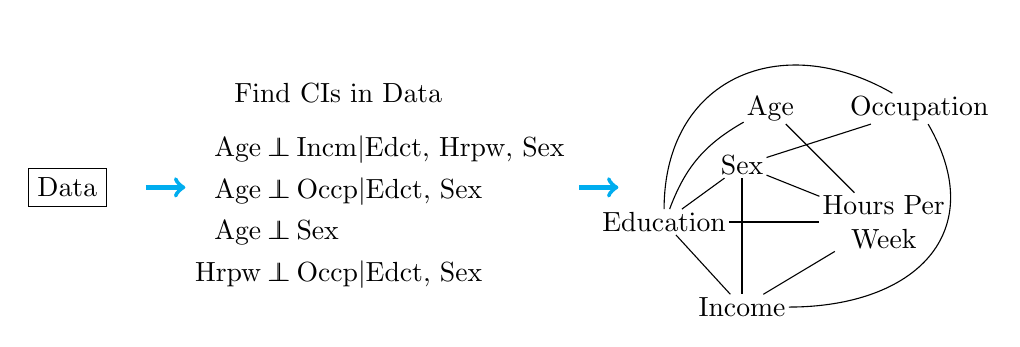
\begin{tikzpicture}
			\node[draw, rectangle] (data) at (0, 0) {Data};
			\draw[ultra thick,->, cyan] (1,0) -- (1.5,0);
			\node[rectangle, align=center, inner sep=1pt] at (3.5, 0) {
				\begin{minipage}{0.3\textwidth}
					\center{\textnormal{Find CIs in Data}}
					\begin{equation*}
						\begin{split}
							\textnormal{Age} &\ci \textnormal{Incm} \rvert \textnormal{Edct, Hrpw, Sex} \\
							\textnormal{Age} &\ci \textnormal{Occp} \rvert \textnormal{Edct, Sex} \\
							\textnormal{Age} &\ci \textnormal{Sex} \\
							\textnormal{Hrpw} &\ci \textnormal{Occp} \rvert \textnormal{Edct, Sex} \\
						\end{split}
					\end{equation*}
				\end{minipage}
				};
			\begin{scope}[xshift=6.5cm]
				\draw[ultra thick,->,cyan] (0,0) -- (0.5,0);
			\end{scope}	
			\begin{scope}[xshift=9.2cm, yshift=1cm, scale=0.9]
				\tikzstyle{every node}=[align=center, inner sep=1pt]
				\node (sex) at (-0.7, -0.8) {Sex};
				\node (age) at (-0.3, 0) {Age};
				\node (ed) at (-1.8, -1.6) {Education};
				\node (occ) at (1.8, 0) {Occupation};
				\node (hrpw) at (1.3, -1.6) {Hours Per \\ Week};
				\node (income) at (-0.7, -2.8) {Income};
			
				\draw[-]  (age) to[bend right=20] (ed);
				\draw[-]  (sex) to (ed);
				\draw[-]  (age) to (hrpw);
				\draw[-]  (ed) to (hrpw);
				\draw[-]  (sex) to (hrpw);
				\draw[-]  (ed) to (income);
				\draw[-]  (hrpw) to (income);
				\draw[-]  (occ) to[out=300, in=0, looseness=1.4] (income.east);
				\draw[-]  (sex) to (income);
				\draw[-]  (ed) to[out=90, in=150, looseness=1.3] (occ);
				\draw[-]  (sex) to (occ);	
			\end{scope}
		\end{tikzpicture}
	\end{figure}

	\center{Unsupervised learning problem: No ground truth DAG.}
\end{frame}

\begin{frame}{Problems with Causal Discovery}
	\center{Main Idea: Quantify information shared between two CI tests.}
	\vspace{1em}
	\begin{itemize}
		\item Many CI tests are dependent on each other
		\item p-value adjustment dependent on how much information is shared between tests.
		\item Test dependence can lead to multiple errors due to the same perturbation in finite samples.
		\item To capture model uncertainty, we need to consider the dependence between CI tests.
	\end{itemize}
	\vspace{1em}

\end{frame}

\begin{frame}{Problem Statement}
	\center{How do we evaluate the performance of a causal discovery algorithm?}
\end{frame}

\begin{frame}{Empirical Results}
	\begin{figure}
		\includegraphics[scale=0.12]{imgs/empirical1.png}
	\end{figure}
\end{frame}

\begin{frame}{Empirical Results}
	\begin{figure}
		\includegraphics[scale=0.12]{imgs/empirical2.png}
	\end{figure}
\end{frame}

\end{document}
